\documentclass{beamer}

\usetheme{Warsaw}
\setbeamerfont*{frametitle}{size=\normalsize,series=\bfseries}
\setbeamertemplate{navigation symbols}{}
%\usefonttheme{professionalfonts}

\usepackage{listings,bera}
\usepackage[english]{babel}
\usepackage[utf8x]{inputenc}
\usepackage{times}
\usepackage[T1]{fontenc}
\usepackage{ulem}
\usepackage{listings}
\usepackage{textcomp}
\usepackage{graphicx}
\usepackage{subfigure}
\usepackage{hyperref}

%\definecolor{fore}{RGB}{249,242,215}
%\definecolor{back}{RGB}{51,51,51}
%\definecolor{title}{RGB}{255,0,90}
%\setbeamercolor{titlelike}{fg=title}
%\setbeamercolor{normal text}{fg=fore,bg=back}

\definecolor{keywords}{RGB}{255,0,90}
\definecolor{comments}{RGB}{60,179,113}
\definecolor{strings}{RGB}{60,179,60}
\definecolor{numbers}{RGB}{179,60,60}
\lstset{language=Python,
        extendedchars=false,
        keywordstyle=\color{keywords},
        commentstyle=\color{comments}\emph,
        stringstyle=\color{strings},
        escapechar=!
        }

% adds the \MongoLogo command to put the logo on a slide
\usepackage[absolute,overlay]{textpos}
\setlength{\TPHorizModule}{1mm}
\setlength{\TPVertModule}{1mm}
\newcommand{\MongoLogo}{
\begin{textblock}{14}(2.0,0.7)
  
\includegraphics[height=0.8cm]{logo-mongodb-ondark.png}
\end{textblock}
}

\pgfdeclareimage[height=2in]{featuregraph}{featuresPerformance.png}
\pgfdeclareimage[height=2.5in]{sharding}{sharding.png}

\title{Document-Oriented DBs and MongoDB}
%\subtitle{What we are and what we aren't}
\author{Mathias Stearn}
\institute{10gen}
\date{VolcaNoSQL EU -- April 20, 2010}

\AtBeginSection[]
{
  \begin{frame}<beamer>{}
    \MongoLogo
    \tableofcontents[currentsection]
  \end{frame}
}


\begin{document}

\begin{frame}
  \MongoLogo
  \titlepage
\end{frame}

\begin{frame}
  \MongoLogo
  \tableofcontents
\end{frame}

\section{Document Oriented Databases}

\begin{frame}
  \MongoLogo
  \begin{itemize}
    \item Only Two Document Oriented DBs Right Now
    \begin{itemize}
      \item MongoDB and CouchDB
      \item Everyone has an opinion on what makes a DODB
      \begin{itemize}
        \item Hard to choose ``defining'' characteristics
        \item This is my take on the space -- deal with it
      \end{itemize}
    \end{itemize}
  \end{itemize}
\end{frame}

\subsection{What they are}
\begin{frame}[fragile]
  \MongoLogo
  \begin{itemize}
    \item Document Oriented
    \begin{itemize}
      \item Think JSON Documents, not Word/OOo Documents
      \item Can store files through Attachments and GridFS
      \item Could use XML but XML sucks
    \end{itemize}
  \end{itemize}

  \begin{lstlisting}
{
  _id: "mstearn",
  name: "Mathias Stearn",
  karma: 42,
  active: true,
  birthdate: new Date(517896000000),
  interests: ["MongoDB", "Python", "!\color{strings}Üñíçøđĕ!"],
  subobjects: [{foo: "bar"},
               {foo: "baz", count: 13}]
}
  \end{lstlisting}
\end{frame}

\begin{frame}[fragile]
  \MongoLogo
  \begin{itemize}
    \item Hierarchical 
    \begin{itemize}
      \item Can nest objects to arbitrary depth
      \item Server can reach into objects
      \item Whole ``Object'' stored at one place on disk
    \end{itemize}
  \end{itemize}

  \small
  \begin{lstlisting}
{
  comments: [
    { by: 'mstearn', body: 'text', tags: ['empty']
        votes: {good: 100, bad: 10, net: 90} },
    { by: 'mdirolf', body: 'what?', tags: ['question']
        votes: {good: 30, bad: 40, net: -10} }
  ]
}
  \end{lstlisting}
\end{frame}

\subsection{What they aren't}
\begin{frame}
  \MongoLogo

  \begin{itemize}
    \item Not Relational
    \begin{itemize}
      \item Not forced into rows/columns/tables
      \item No built-in joins
        \begin{itemize}
          \item Less need because objects can directly store lists
        \end{itemize}
      \item Many-to-Many still possible (learn how at workshop)
      \item No SQL (no SQL injections either)
      \item No Object-Relational impedance mismatch
    \end{itemize}
  \end{itemize}
\end{frame}

\begin{frame}
  \MongoLogo

  \begin{itemize}
    \item Not Just Key-Value Store
    \begin{itemize}
      \item Key and value are not separate
      \item Supports queries on non-primary keys
        \begin{itemize}
          \item Secondary Indexes
        \end{itemize}

      \item Supports Aggregation
        \begin{itemize}
          \item Currently via JavaScript MapReduce
          \item Both DBs looking into alternatives
        \end{itemize}
        
      \item Can be as fast as a KV store if you only need KV features
        \begin{itemize}
          \item But still have access to a real database when needed
        \end{itemize}

      \item Less custom code needed
    \end{itemize}
  \end{itemize}
\end{frame}

\begin{frame}
  \MongoLogo

  \begin{itemize}
    \item Not the same as stuffing a JSON blob in a database
    \begin{itemize}
      \item Database understands document format
      \item Can query on any field
      \item ``Use the right tool for the job''
    \end{itemize}
  \end{itemize}
\end{frame}

\section{CouchDB}
\begin{frame}[fragile]
  \MongoLogo

  \begin{block} {\color{red}WARNING}
    I am not an expert on CouchDB!
  \end{block}
\end{frame}

\subsection{Pros and Cons}
\begin{frame}[fragile]
  \MongoLogo

  \begin{block} {Pros}
    \begin{itemize}
      \item HTTP RESTful Interface
      \item Stores and communicates in plain JSON
      \item Query using precomputed JS Map/Reduce views
      \item Fastest if you use Bulk Insert
      \item Uses Append-Only File
    \end{itemize}
  \end{block}
\end{frame}

\begin{frame}[fragile]
  \MongoLogo

  \begin{block} {Cons}
    \begin{itemize}
      \item HTTP RESTful Interface
      \item Stores and communicates in plain JSON
      \item Query using precomputed JS Map/Reduce views
      \item Fastest if you use Bulk Insert
      \item Uses Append-Only File
    \end{itemize}
  \end{block}
\end{frame}



\section{MongoDB}
\subsection{Compared to CouchDB}
\begin{frame}[fragile]
  \MongoLogo

  \begin{block} {MongoDB}
    \begin{itemize}
      \item Custom wire protocol with many supported languages
      \item Stores and communicates in BSON (Binary JSON)
      \item Rich Ad-Hoc Query Language 
        \begin{itemize}
          \item MapReduce for aggregation
        \end{itemize}
      \item Bulk Insert available, but regular insert is very fast
      \item Data is updated in place
    \end{itemize}
  \end{block}
\end{frame}


\subsection{Into to Mongo}

\begin{frame}
  \MongoLogo
  \begin{center}
    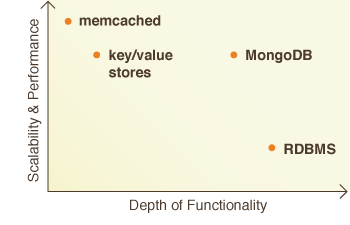
\includegraphics[height=6cm]{featuresPerformance.png}
  \end{center}
\end{frame}

\begin{frame}[fragile]
  \MongoLogo
  \begin{itemize}
    \item The Mongo Shell
      \begin{itemize}
        \item \url{http://try.mongodb.org} ${\leftarrow}$ go here now
      \end{itemize}
    \item Full JS shell + MongoDB extensions
    \item Most MongoDB documentation uses shell syntax
  \end{itemize}
\end{frame}

\begin{frame}[fragile]
  \MongoLogo

  \small
  \begin{lstlisting}[numbers=left, numberstyle=\tiny\color{red}]
db.users.insert({_id:'mstearn',
                 name: {first:'Mathias',
                        last:'Stearn'}
                 company: '10gen',
                 knows: ['MongoDB', 'Python', 'C++'],
                 posts: 42})
                 
db.users.find({_id: 'mstearn'})
db.users.find({company: '10gen'})
db.users.find({posts: {$gte: 40, $lt: 50}}) 
db.users.find({'name.last': 'Stearn'})
db.users.ensureIndex({knows: 1})
db.users.find({knows: 'MongoDB'})
db.users.find({knows: {$in: ['MongoDB', 'Mongo']}})
db.users.find({knows: {$all: ['MongoDB', 'Python']}})
db.users.find({knows: /^Mongo/})
db.users.find().sort({posts: -1}).skip(10).limit(10)
  \end{lstlisting}
\end{frame}


\begin{frame}[fragile]
  \MongoLogo

  \begin{block}{Shameless self-promotion}
    \url{http://github.com/RedBeard0531/MongoMagic/}
  \end{block}

  \begin{lstlisting}[numbers=left, numberstyle=\tiny\color{red}]
db.users.find( M._id == 'mstearn' )
db.users.find( M.company == '10gen' )
db.users.find( 40 <= M.posts < 50 ) 
db.users.find( M.name.last == 'Stearn' )
db.users.find( M.knows.IN('MongoDB', 'Mongo') )
db.users.find( M.knows.ALL('MongoDB', 'Python') )
db.users.find( M.knows.STARTSWITH('Mongo') )
  \end{lstlisting}
\end{frame}
\begin{frame}[fragile]
  \MongoLogo

  \small
  \begin{lstlisting}[numbers=left, numberstyle=\tiny\color{red}]
db.zips.insert({_id: '10011', loc: [43, -74]})

db.zips.ensureIndex({loc: '2d'})

db.zips.find({loc: {$near: [43, -74]}})

var box = [[x1, y1], [x2, y2]]
db.zips.find({loc: {$within: {$box: box}}})

var circle = [[x,y], radius]
db.zips.find({loc: {$within: {$center: circle}}})
                 
  \end{lstlisting}
\end{frame}

\begin{frame}[fragile]
  \MongoLogo

  \small
  \begin{lstlisting}[numbers=left, numberstyle=\tiny\color{red}]
db.posts.insert({_id: ObjectId(123),
                 by: 'mstearn',
                 title: 'Why MongoDB is Awesome',
                 body: 'It just is MASSIVE TYPO',
                 tags: [] })

db.posts.update({_id: ObjectId(123)},
                {$set: {body: 'It just is' }})

db.posts.update({_id: ObjectId(123)},
                {$push: {tags: 'Citation Needed'}})

db.tags.update({_id: 'Citation Needed'},
               {$inc: {count: 1}},
               {upsert: true})
  \end{lstlisting}
\end{frame}

\subsection{Sharding}
\begin{frame}[fragile]
  \MongoLogo
  \begin{itemize}
    \item You {\tiny (probably)} don't need sharding!

    \item My desktop can handle 100k inserts/s or 160k queries/s
      \begin{itemize}
        \item For comparison, linkedin gets 55M views/day [quantcast]
        \item $55000000 / 8 / 60 / 60 = 1736$ views/sec
      \end{itemize}

    \item Largest Mongo install is 12TB on single server
      \begin{itemize}
        \item Mostly large objects
      \end{itemize}

    \item Wordnik.com has 1.5TB in over 5 Billion docs
      \begin{itemize}
        \item Sustained 100,000 inserts per second during loading
        \item Queries are 4x faster than old MySQL setup
      \end{itemize}

    \item Speed and Scalability are different things
      \begin{itemize}
        \item But you only need scalability if you're too slow
      \end{itemize}

  \end{itemize}
\end{frame}

\begin{frame}
  \MongoLogo
  \center
  \pgfuseimage{sharding}
\end{frame}

\begin{frame}
  \MongoLogo

  \center {\huge Questions?}

  \begin{block}{Links}
  \begin{itemize}
    \item http://media.mongodb.org/zips.json (for workshop)
    \item http://try.mongodb.org (Try mongo in your browser)
    \item http://www.mongodb.org
    \item \#mongodb on irc.freenode.net
    \item mongodb-user on google groups
  \end{itemize}
  \end{block}

  \begin{block}{Contact}
  \begin{itemize}
    \item mathias@10gen.com
    \item @mathias\_mongo ${\leftarrow}$ follow me!
  \end{itemize}
  \end{block}
\end{frame}

\end{document}

% vim: set softtabstop=2
